This section is structured as follows:
First, we give a general overview of the results of our survey in Subsection~\ref{genoverview}.
Thereafter, we depict and discuss a conceptualisation of the data quality domain followed by a formal definition of the terminologies related to data quality in detail in Subsection~\ref{concepts}.
A quantitative evaluation of our literature review is presented in the Subsection~\ref{qntyeval} followed by a qualitative evaluation in Subsection~\ref{qltyeval}.

\subsection{General Overview}
\label{genoverview}
%Distinction between methodologies used in Linked Data and Database communities based on Open and Closed World Assumption

\subsection{Conceptualization}
\label{concepts}
\paragraph{Definition of Terminologies.}
A generalized architecture of data quality is depicted in Figure. 
There exist a number of discrepancies in the definition of many concepts, especially in data quality due to the contextual nature of quality~\cite{Batini:2006} .
Therefore, in the sequel we describe and formally define the research context terminology as well as individual components and concepts in more detail.

\textbf{RDF Dataset.}
%In this document, we understand a data source as an access point for Linked Data in the Web. It provides a dataset and it may support multiple methods of access.

The RDF triples, RDF graph and the RDF datasets have been adopted by the W3C Data Access Working Group \cite{Las99,Hayes:2004,Brickley-2004}

Given an infinite set $\mathcal{U}$ of URIs (resource identifiers), an infinite set $\mathcal{B}$ of blank nodes, and an infinite set $\mathcal{L}$ of literals, a triple $ \langle s, p, o \rangle \in (\mathcal{U} \cup \mathcal{B})\times \mathcal{U} \times (\mathcal{U} \cup \mathcal{B} \cup \mathcal{L})$ is called an RDF triple; $s$, $p$, $o$ are called, respectively, the subject, the predicate and the object of the triple. An RDF graph $G$ is a set of RDF triples. A named graph is a pair  $\langle G,u \rangle$, where $G$ is called the default graph and $u\in\mathcal{U}$. An RDF dataset is a set of default and named graphs = $\lbrace G, (u_1,G_1), (u_2,G_2), ...(u_n,G_n)\rbrace$. 

\textbf{Data Quality.}
%WIQA

The concept of data quality is a domain-specific subconcept of the general concept of quality. 
A popular definition for quality is the "fitness for use"~\cite{qdefn}.
Data quality is commonly conceived as a multidimensional construct, as the "fitness for use" may depend on various factors such as accuracy, timeliness, completeness, relevancy, objectivity, believability, understandability, consistency, conciseness, availability, and verifiability~\cite{qconsumers}.
In terms of the semantic web, there are varying concepts of data quality.
The semantic metadata, for example, is an important concept to be considered when assessing the quality of datasets~\cite{Leigold}.
On the other hand, the notion of link quality is another important aspect in Linked Data that is introduced, where it is automatically detected whether a link is useful or not~\cite{Gueret}.
Also, it is to be noted that \textit{data} and \textit{information} are interchangeably used in the literature. 

\textbf{Data Quality Problems.}
%What is data quality problem? How the others have defined it?

The data quality problem refers to a set of issues that can affect the potentiality of the applications that use data. 
In the literature there is no such a specific definition related to data quality problems. In \cite{Flemming} the author does not provide a definition of it but implicitly explains that in terms of \textit{data diversity}. In \cite{Hogan} the authors discuss about \textit{errors} or \textit{noise} or \textit{difficulties} and in \cite{Hogan:2012} the author discuss about \textit{modelling issues} which are prone of the non exploitations of those data from the applications.

Bizer et al. \cite{Bizer} defines the data quality problems as a choice of the web-based information systems design which integrate information from different providers.  In \cite{Mendes} the problem of data quality is related to values being in conflict between different data sources as as a consequence of the diversity of the data. 

%because it may be incomplete, poorly formatted, inconsistent,
%What kind of problems we could have?
%Errors which compromise the effectiveness of applications leveraging the resulting data. 
%- Publishing errors; Incomplete; Incoherent; Poorly formatted; Inconsistent; Hijack; Dereferancability; Syntax errors; Link quality; Outdated; Incorrectness; Serialization problems; Inusability; System Problems; Inaccurate; Misleading; Outdated\\

%Semantic Metadata
%Data sources my have low quality such as misspelling, erroneous statements, etc; problems could be derived from the heterogeneity of data sources such as inconsistencies and duplicated entries; or be introduces by the tools employed. Changes to the data sources or to the underlying ontologies could also bring problems. 
%data are modelled in a manner that is not
%facilitative to generic consumption

\textbf{Data Quality Criteria.}
%dimension, criteria
%indicators, metric, measures

Data quality assessment involves the measurement of quality \textit{dimensions} or \textit{criteria} that are relevant to the consumer.
A data quality assessment \textit{metric} or \textit{measure} is a procedure for measuring an information quality dimension~\cite{Bizer}. 
These metrics are heuristics that are designed to fit a specific assessment situation~\cite{metric}.
Since the criteria are rather abstract concepts, the assessment metrics rely on quality \textit{indicators} that allow for the assessment of the quality of a data source w.r.t the criteria~\cite{Flemming}.
An assessment score is computed from these indicators using a scoring function. 

The data quality assessment metrics can be classified into three categories according to the type of information that is used as quality indicator: (1) Content Based - information content itself; (2) Context Based - information about the context in which information was claimed; (3) Rating Based - based on the ratings about the data itself or the information provider~\cite{Bizer}. 

\textbf{Data Quality Assessment Method.}
%WIQA

A data quality assessment methodology is defined as the process of evaluation if a piece of data meets in the information consumers need in a specific use case~\cite{Bizer}.
The process involves measuring the quality dimensions that are relevant to the user and comparing the assessment results with the users quality requirements.
The steps involved in data quality assessment are: (1) formulating a research question; (2) selecting datasets and perf``xorming analyses; (3) detecting quality problems; (4) performing data quality analysis; (5) improving data quality and identifying short comings.
%Semantic Metadata
%There are three major steps involved in the evaluation procedure, including: setting up the evaluation context, detecting quality problems and calculating and analyzing the quality status. 

\begin{figure}
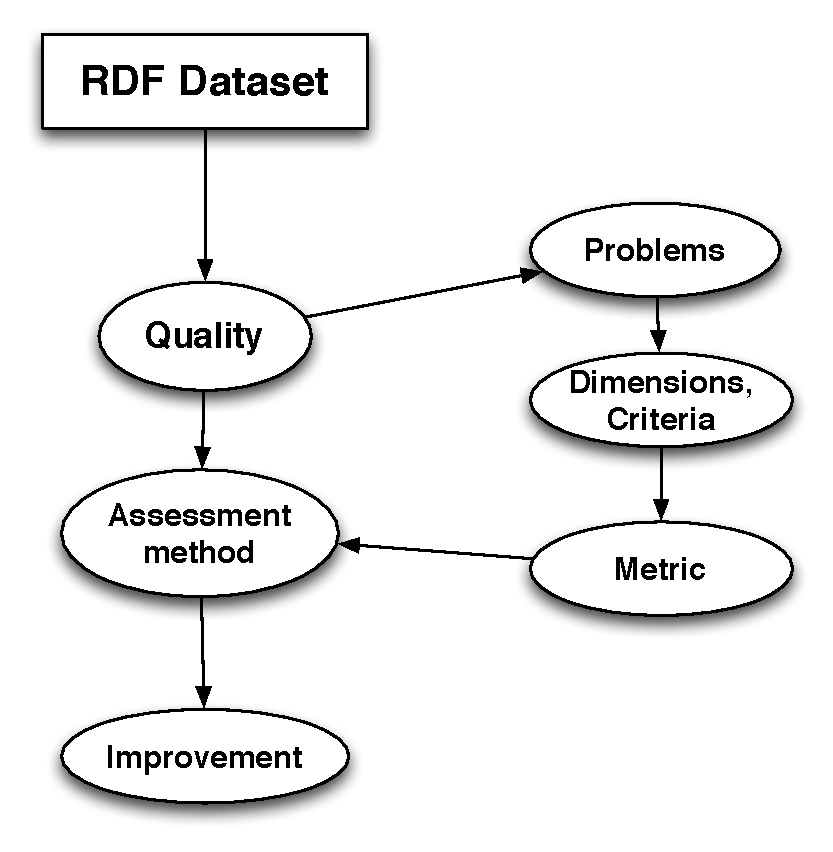
\includegraphics[scale=0.5]{Mindmap.pdf}
\caption{Conceptualization of the data quality domain.}
\label{fig:lod-life-science}
\end{figure}

\subsection{Quantitative Evaluation}
\label{qntyeval}
Out of the total number of articles retrieved from the initial literature survey, most were only related to the general aspects of data quality assessment of the data available on the Web. After refining our search strategy by using a combination of keywords and the advanced search forms available for most of the online databases, we retrieved (no.?) of articles. After reading through the articles in detail, only 9 were identified to be specifically those reporting a methodology or framework for data quality assessment of Linked Data.

%Out of the 9 articles, (no.) are from the year (?), (conference/journal).

Additionally, those articles related to provenance quality assessment, were also retrieved. A total number of (48?) articles were identified. 

\subsection{Qualtitative Evaluation}
%http://goo.gl/s2wq1
\label{qltyeval}

This section on the qualitative evaluation of the articles consists of: (i) an evaluation of each of the framework in terms of their application field, goal, target data and degree of automation of the tool, if provided; (ii) a comprehensive list of the data quality dimensions and their occurrence in the papers followed by a combination of definitions provided by several authors; (iii) a list of data quality metrics used for each of the dimensions that have been used in the papers and (iv) a generalisation of the data quality assessment steps that are followed by most authors including an account of the input and output for each step, whether a tool exists and the involvement of the user for each tool.  

\subsubsection{Qualitative evaluation of frameworks}

Table~\ref{appfield}

\begin{itemize}
\item Application field: related to whether the application covers a specific use case or covers every use case in different domains. 
\item Type of data: related to the fine grained of the data used from each paper such as triples, resources, two or more data sources and entire LOD cloud. 
\item Degree of a automation: related to the degree of interaction of the users to using the tool such as manual, semi-automated, automated. 
\end{itemize}

From the evaluation, it is observed that five out of the 20 papers focus on a very specific application or a particular domain. 
Majority of the papers develop frameworks or methodologies for the assessment of published data. 
However, most of the methodologies are only applicable at the triple or resource level. 
Six approaches, on the other hand, can be applied to two or more resources and to the entire LOD cloud.
Eight of the approaches have also implemented a tool, which is available for users to assess the quality of the LOD datasets.
The degree of automation also varies for these various tools. 
Majority of them are semi-automated or automated, two of them namely Sieve and WIQA, require a considerable amount of manual configuration and therefore requires a large amount of user involvement.  

%Then we should go into detail and describe some tool which is really useful like Flemming and Sieve and also talk about the Provenance papers in detail

\onecolumn
\begin{landscape}
\begin{table*}
\caption{Qualitative evaluation of frameworks} \label{appfield}
\begin{tabular}{ p{2.3cm} c p{7cm}  c  p{0.9cm} l p{1cm} l p{0.7cm} l cp{0.5cm} }
\hline
\textbf{Paper} & {\textbf{Application}} & \textbf{Goal} & \multicolumn{4}{c}{\textbf{Type of data}} & \multicolumn{3}{c}{\textbf{Degree of automation}} & \textbf{Tool support} \\
%\cline{2-4}
\hline
 & \textbf{G}eneral/\textbf{S}pecific &  & \textbf{Triple} & \textbf{Resource} & \textbf{Several resources} & \textbf{Entire LOD Cloud} & \textbf{Manual} & \textbf{Semi-automated} & \textbf{Automated} & \\
\hline
Bizer et.al., 2009 & G  & Information filtering & \tick & \tick & \tick & -  & \tick &  - & - & \tick \\
\hline
B\"ohm et.al., 2010 & G  & Data integration & \tick & \tick & - & - &  & \tick & -  & \tick \\
\hline
Chen et.al., 2010  & G  & Generating semantically valid hypothesis & \tick & \tick & - & - & - & - & - & - \\
\hline
Flemming et.al., 2010 & G  & Assessment of published data & \tick & \tick & - & - & - & \tick & - & \tick \\
\hline
Gu\'eret et.al., 2011 & S & Assessment of quality of links & - & - & - & \tick & - & - & \tick & \tick \\
\hline
Hogan et.al., 2010 & G &Assessment of published data by identifying RDF publishing errors and providing approaches for improvement & \tick & \tick & \tick &\tick & - & \tick & - & \tick \\
\hline
Hogan et.al., 2012 & G & Assessment of published data & \tick & \tick & \tick &\tick & - & - & - & - \\
\hline
Lei et.al., 2007 & S & Assessment of semantic metadata & \tick & \tick & - & - & - & - & - & - \\
\hline
Mendes et.al., 2012 & S & Data integration & \tick & - & - & - & \tick & - & - & \tick \\
\hline
Mostafavi et.al., 2004& S & Spatial data integration & \tick & \tick & - & - & - & - & - & - \\
\hline
Hartig, 2009 & G & Provenance model for RDF data & \tick & - & - & - & - & \tick & - & \tick \\
\hline
Hartig et.al., 2009& G & Assessment of published data using provenance information about the data on the Web to assess the quality and trustworthiness. & \tick & \tick & - & - & - & - & - & - \\
\hline
Gamble et.al., 2011& G & Application of decision networks to quality, trust
and utility assessment & - & - & \tick & \tick & - & - & - & - \\
\hline
Shekarpour et.al., 2008 & G & Method for evaluating trust & - & - & \tick & \tick & - & - & - & - \\
\hline
Golbeck et.al., 2006 & G & Algorithm for computing personalized trust recommendations using the provenance of existing trust annotations in social networks & - & - & \tick & \tick & - & - & - & - \\
\hline
Gil et.al., 2002 & G & Approach to derive an assessment of a data source
based on the annotations of many individuals & \tick & \tick & - & - & - & \tick & - & \tick \\
\hline
Golbeck et.al., 2003 & G & Trust networks on the semantic web & - & \tick & - & - & - & - & - & - \\
\hline
Gil et.al., 2007 & S & Trust assessment of web resources & - & \tick & - & - & - & - & - & - \\
\hline
Jacobi et.al., 2011 &  G & Trust assessment of web resources & - & \tick & - & - & - & - & - & - \\
\hline
Hartig et.al., 2010 & G & Trust assessment of web resources & - & \tick & - & - & - & - & - & - \\
\hline
\end{tabular}
\end{table*}
\end{landscape}
\twocolumn

\subsubsection{Data quality dimensions}

Dimensions: related to the quality dimensions identified in each work to abstractly assess data quality in LOD. 
It is possible to define a basic set of data quality dimensions, including accuracy, completeness, consistency, and timeliness, which constitute the focus of the majority of authors: 
\begin{itemize}
\item Accuracy 
%Amrapali
\item Consistency
%Anisa
\item Coherence
%Amrapali
\item Provenance
%Anisa
\end{itemize}

Table~\ref{dimex} contains a comprehensive list of the data quality dimensions and their respective definitions provided by several authors.

Table~\ref{dimensions} shows the occurrence of each dimension in the included articles. 


\begin{table*}[htb]
\caption{Data quality dimensions and their definitions.} 
\label{dimex}
\begin{tabular}{ | p{2cm} | p{12cm} | }
\hline
\textbf{Accuracy} & "the degree of correctness and precision with which information in an information system represents states of the real world." \cite{Bizer} \\
\hline
\textbf{Consistency} & "implies that two or more values do not conflict with each other." \cite{Bizer}
"The consistency criterion contains aspects indicating contradictions in the data. It can be seen a prerequisite for the correctness of the data, as inconsistent values cannot all be correct." \cite{Flemming}
"inconsistent: a software agent will interpret a contradiction in the data." \cite{Hogan}
"The deficiency identified in this category is inconsistent representation, which denotes the situation where an instance is inconsistent with the ontologies." \cite{Lei}
"A data set is consistent if it is free of conflicting information." \cite{Mendes} \\
\hline
\textbf{Objectivity} & "Objectivity is the extent to which information is unbiased, unprejudiced and impartial." \cite{Bizer} \\
\hline

\textbf{Timeliness} & "Timeliness is the degree to which information is up-to-date." \cite{Bizer}
"The timeliness criterion refers to the currentness of the data provided by a source. It is part of the correctness of the data, as outdated data might meanwhile have become invalid." \cite{Flemming}" \\
\textbf{TimeCloseness} measures the distance between the input date from the provenance graph to the current date, with more recent data receive scores closer to 1." \cite{Mendes}

In \cite{Rula}, the authors do not provide a \textit{mirefillte} definition of timeliness but they provide a definition of currency, another quality dimensions related to time, which is \textit{huazuar} from the data quality domain as "Currency is defined as a measure of the age of data" and furthermore they provide a measure of currency at document and graph level. For instance, lets consider we want to evaluate the age of the following statement: X ceoOf Y. Considering the approach we can deduce from the age of the 


\hline
\textbf{Believability} & "The extent to which information is regarded as true and credible.| \cite{Bizer} \\
\hline
\textbf{Completeness} & "Completeness is the degree to which information is not missing. Schema completeness which is the degree to which entities and attributes are not missing in a schema; column completeness which is a function of the missing values in a column; and population completeness which refers to the ratio of entities represented in an information system to the complete population." \cite{Bizer}
"incomplete: equatable to a dead-link in the current HTML web, a software agent will not be able to retrieve data relevant to a particular task." \cite{Hogan}
"On the schema level, a data set is complete if it contains all of the attributes needed for a given task. On the data(instance) level, a data set is complete if it contains all of the necessary objects for a given task." \cite{Mendes} \\
\hline
\textbf{Understandibility} & "Understandability is the extent to which data is easily comprehended by the information consumer." \cite{Bizer}
"A third criterion relating to the representation of the data is its comprehensibility, i.e. the ease with which human consumers can understand and utilize the data." \cite{Flemming} \\
\hline
\textbf{Relevancy} & Relevancy is the extent to which information is applicable and helpful for the task at hand. (Bizer) \\
\hline
\textbf{Reputation} &  \\
\hline
\textbf{Verifiability} & "Verifiability is the degree and ease with which the information can be checked for correctness." \cite{Bizer}
"The verifiability criterion refers to the means a consumer is provided with, which can beused to examine the data for correctness. Without such means, the only way of having a certain assurance of the correctness of the data is the consumer's trust in the source." \cite{Flemming} \\
\hline
\textbf{Amount of data} & "Amount of Data is the extent to which the volume of data is appropriate
for the task at hand." \cite{Bizer}
Another criterion inluencing the usability of a data source is the amount of data it provides. Although a main advantage of the Web of Data compared to the traditional web is the possibility to aggregate data from several sources, the necessity to match the underlying vocabularies puts that advantage into perspective. Thus, larger datasets should be preferred." \cite{Flemming}
"whether the amount of collected data is appropriate: If the collected data is not enough to approximate the �true� scenario precisely, we will get many wrong or coincident rules (false negative)." \cite{Chen} \\
\hline
\textbf{Rep.Consistency} & "extent to which information is compactly represented" \cite{Bizer}. "Issues related to the format (part of syntax)" \cite{} \\
\hline
\textbf{Rep.Conciseness} & is the extent to which information is in appropriate languages, symbols, and units, and the definitions are clear (Bizer). Issues related to meaning (part of semantic), e.g. currency in dollars and in jens   \\
\hline
\textbf{Availability} & "extent to which information is available, or easily and quickly retrievable." \cite{Bizer}. "refers to the proper functioning of all access methods." \cite{Flemming}\\
\hline
\textbf{Response Time} & "measures the delay between submission of a request by the user and reception of the response from the system." \cite{Bizer}. \\
\hline
\textbf{Security} &  \\
\hline
\textbf{Uniformity} & "refers to the usage of established techniques in order to increase the usability of the data." \cite{Flemming} \\
\hline
\textbf{Versatility} & "refers to alternative representations of the data and its handling." \cite{Flemming} \\
\hline
\textbf{Validity of documents} & "consists of two aspects influencing the usability of the documents: the valid usage of the underlying vocabularies and the valid syntax of the documents." \cite{Flemming} \\
\hline
\textbf{Licensing} & "without a licence, the data consumer cannot legally use the data as intended." \cite{Flemming} \\
\hline
\textbf{Performance} & "comprises aspects of enhancing the performance of a source as well as measurings of the actual values." \cite{Flemming} \\
\hline
\textbf{Conciseness} & "On the schema level, a dataset is concise if it does not contain redundant attributes (two equivalent attributes with different names). On the data (instance) level, a data set is concise if it does not contain redundant objects (two equivalent objects with different identifiers). The extensional conciseness measures the number of unique objects in relation to the overall number of object representations in the dataset." \cite{Mendes} \\
\hline
\textbf{Coherence} & \\
\hline
\textbf{Provenance} & \\
\hline
\end{tabular}
\end{table*}

\onecolumn
\begin{landscape}
%\begin{table*}[htb]
%\begin{center}
\begin{longtable}{ | p{2.3cm} | p{0.6cm} | p{0.65cm} | p{0.55cm} | p{1.27cm} | p{0.8cm} | p{0.73cm} | p{0.75cm} | p{0.55cm} | p{0.9cm} | p{1.2cm} | p{0.77cm} | p{0.7cm} | p{0.9cm} | p{1.4cm} | p{1cm} | p{0.6cm} | p{1cm} | p{0.6cm} | }
\caption{A list of data quality dimensions and their usage in each of the included papers.} 
\label{dimensions} \\
\hline
\textbf{Dimensions} & Bizer et.al., 2009 & B\"ohm et.al., 2010 & Chen et.al., 2010 & Flemming et.al., 2010 & Gu\'eret et. al, 2011& Hogan et.al., 2010 & Hogan et.al., 2012& Lei et.al., 2007& Mendes et.al., 2012 & Mostafavi et.al., 2004 & Hartig, 2009 & Hartig et.al., 2009	& Gamble et.al., 2011 & Shekarpour et.al., 2008 & Golbeck et.al., 2006 & Gil et.al., 2002 & Golbeck et. al., 2003 & Gil et.al., 2007\\
\hline
\textbf{Accuracy} & \tick & \tick & & & \tick & & & \tick & & & & & & & & & & \\
\hline
\textbf{Consistency} & \tick & \tick & \tick & \tick & & \tick & & \tick & \tick & \tick & & & & & & & & \\
\hline
\textbf{Objectivity} & \tick & & & & & & & & & & & & & & & & & \\
\hline
\textbf{Timeliness} & \tick & & & \tick & & & & \tick & \tick & & & & & & & & & \\
\hline
\textbf{Believability} & \tick & & & & & & & & & & & & & & & & & \\
\hline
\textbf{Completeness} & \tick & & & & \tick & \tick & & & \tick & & & & & & & & & \\
\hline
\textbf{Understand - ibility} & \tick & & & \tick & & & & & & & & & & & & & & \\
\hline
\textbf{Relevancy} & \tick & & & & & & \tick & & & & & & & & & & & \\
\hline
\textbf{Reputation} & \tick & & & & & & & & \tick & & & & & & & & & \\
\hline
\textbf{Verifiability} & \tick & & & \tick & & & & & & & & & & & & & & \\
\hline
\textbf{Amount of data} & \tick & & \tick & \tick & & & & & & & & & & & & & & \\
\hline
\textbf{Accuracy} & & & & & & & & & & & & & & & & & & \\
\hline
\textbf{Interpretability} & \tick & & & & & & \tick & & & & & & & & & & & \\
\hline
\textbf{Rep.Conciseness} & \tick & & & & & & \tick & & & & & & & & & & & \\
\hline
\textbf{Rep.Conssitency} & \tick & & & & & & \tick & & & & & & & & & & & \\
\hline
\textbf{Availability} & \tick & & & \tick  & & & \tick & & & & & & & & & & & \\
\hline
\textbf{Response Time} & \tick  & & & & & & & & & & & & & & & & & \\
\hline
\textbf{Security} & \tick  & & & & & & & & & & & & & & & & & \\
\hline
\textbf{Uniformity} & & & & \tick  & & & & & & & & & & & & & & \\
\hline
\textbf{Versatality}& & & & \tick  & & & & & & & & & & & & & & \\
\hline
\textbf{Validity of documents} & & & & \tick  & & & & & & & & & & & & & & \\
\hline
\textbf{Licensing} & & & & \tick & & & \tick & & & & & & & & & & & \\
\hline
\textbf{Performance} & & & & \tick & & & \tick & & & & & & & & & & & \\
\hline
\textbf{Conciseness} & & & & & & & & & \tick & & & & & & & & & \\
\hline
\textbf{Coherence} & & & & & \tick & & & & & & & & & & & & & \\
\hline
\textbf{Provenance} & & & & & & & & & & & & & & & & & & \\
\hline
%\end{tabular}
%\end{center}
%\end{table*}
\end{longtable}
\end{landscape}
\twocolumn

\subsubsection{Data quality metrics}

Metrics: related to the measurements of each work provided to assess the quality in LOD.
In general, multiple metrics can be associated with each quality dimension.
\textit{ In some cases, the metric is unique and the theoretical definition of a dimension coincides with the operational definition of the corresponding metric. 
For this reason, we make a distinction between theoretical and operational definitions of dimensions only when the literature provides multiple metrics.}
Table~\ref{metrics} provides a list of the data quality metrics for each of the dimensions, how each one can be measured and classifies it as being either subjective or objective.

\onecolumn
%\begin{table*}[htb]
\begin{longtable}{ | p{2.3cm} | p{7.5cm} | m{2cm} |  }
\caption{Comprehensive list of data quality metrics, how they can be measured and the type} 
\label{metrics} \\
\hline
\textbf{Dimension} & \textbf{Metric} & \textbf{Type of metric (Subjective/Objective)} \\
\hline
\multirow{10}{*}{Accuracy} & Interlinking & O \\
& Dereferencabiity issues & O \\
& No structured data available & O \\
& Misreported content types & O \\
& RDF/XML Sytanx errors & O \\
& Spurious annotation/representation & O \\
& Inaccurate annotation & O \\
& Inacurrate labeling and classification & O \\
& detect poor attributes & O \\
& accuracy of interlinking between datasets & O \\
\hline
\multirow{9}{*}{Consistency} & no definitions of entities as being members of disjoint classes & \\
& valid usage of inverse-functional properties & \\
& no redefinition of existing properties & \\
& usage of homogeneous datatypes & \\
& no stating of inconsistent values for properties & \\
& annotation & \\
& reasoning: noise and inconsistency & \\
& misuse of predicates & \\
& inconsistencies in ontologies & \\
\hline
Objectivitiy & no bias or opinion expressed when a data provider interprets or analyses facts & \\
\hline
\multirow{4}{*}{Timeliness} & stating the most recent validation of the data & \\
& no inclusion of outdated data & \\
& inclusion of recent data & \\
& dereferencability of all internal and external URIs & \\
\hline
\multirow{2}{*}{Believability} & meta-information about the identify of information provider & \\
& checking source from which information is retrieved & \\
\hline
\multirow{6}{*}{Completeness} & schema completeness & \\
& column completeness & \\
& population completeness & \\
& URI/HTTP: accessibility and dereferencability & \\
& linking & \\
\hline
\multirow{10}{*}{Understandibility} & human-readable labelling of classes, properties and entities by providing rdfs:label & \\
& human-readable description of classes, properties and entities by providing an rdfs:comment & \\
& indication of metadata about a dataset & \\
& indication of one or more exemplary URIs & \\
& indication of a regular expression that matches the URIs of a dataset & \\
& indication of an exemplary SPARQL query & \\
& indication of some of the vocabularies used & \\
& operability of HTML documents & \\
& provision of message boards and mailing lists & \\
& meta information about the language of web content & \\
\hline
\multirow{5}{*}{Relevancy} & using meta-information attributes & \\
& count occurrence of relevant terms within these attributes & \\
& looking for licensing meta-information like Creative Commons labels & \\
& sort documents according to their relevancy for a given query & \\
& existence of links to external data providers: use external URIs, provide owl:sameAs link & \\
\hline
\multirow{4}{*}{Verifiability} & stating basic provenance information & \\
& usage of a dedicated provenance vocabulary & \\
& usage of digital signatures & \\
& traceability and provability & \\
\hline
\multirow{4}{*}{Amount of data} & no. of triples in a dataset & \\
& no. of internal and external links & \\
& scope and level of detail - coverage & \\
& whether the amount of collected data is appropriate & \\
\hline
\multirow{5}{*}{Interpretability} & use of appropriate language, symbols, unites and clear definitions & \\
& use of self-descriptive formats, identifying objects and terms used to define the objects with globally unique identifiers & \\
& use of various schema languages to provide definitions for terms & \\
& naming resources - avoiding blank nodes & \\
& dereferenced representations - giving human readable metadata & \\
\hline
Rep. Conciseness & information is compactly represented - keep URIs short & \\
\hline
\multirow{3}{*}{Rep. Consistency} & re-use existing terms & \\
& cherry pick vocabularies & \\
& provision of data in different representational formats & \\
\hline 
\multirow{11}{*}{Availability} & accessibiliy of the server & \\
& dereferenceable URIs & \\
& host of stable URIs & \\
& URIs don't contain variable information & \\
& homogeneous (lower) case of URIs & \\
& redirection using the status code 303 See Other & \\
& accessibility of the SPARQL endpoint & \\
& accessibility of the RDF dumps & \\
& URI/HTTP: accessibility and derefencability & \\
& accessibility of the RDF dumps  & \\
& dereferenced representations:�
- dereference forward links
- dereference back-links & \\
\hline
Response time & delay between submission of a request by the user and reception of the response from the system & \\
\hline 
Security & \\
\hline
\multirow{4}{*}{Uniformity} & usage of an established format & \\
& stating the content-types as specifically as possiblet & \\
& usage of established vocabulariest & \\
& referencing of established URIst  & \\
\hline
\multirow{6}{*}{Versatility} & provision of the data in various formats & \\
& provision of the data in various languages & \\
& application of content negotiation & \\
& correct interpretation of the accept-headers sent & \\
& human-readable indication of a SPARQL-endpoint & \\
& machine-readable indication of a SPARQL-endpoint & \\
\hline
\multirow{4}{*}{Validity of documents} & no syntax errors & \\
& exclusive usage of defined classes and properties & \\
& no usage of deprecated classes and properties & \\
& usage of proper datatypes & \\
\hline
\multirow{7}{*}{Licensing} & machine-readable indication of a licence & \\
& human-readable indication of a licence & \\
& permitted reproduction of data & \\
& permitted distribution of data & \\
& permitted modification and redistribution of data & \\
& no attribution needed & \\
& no Copyleft / Share Alike needed & \\
\hline
\multirow{8}{*}{Performance} & machine-readable indication of one or more RDF dumps & \\
& human-readable indication of one or more RDF dumps & \\
& usage of Slash-URIs when providing a large amout of data & \\
& low latency & \\
& high throughput & \\
& only minor variations of the performance & \\
& maintenance of the performance no matter the load & \\
& avoid prolix RDF features & \\
\hline
\multirow{2}{*}{Conciseness} & schema level : intensional conciseness - does not contain redundant attributes & \\
& data level : extensional conciseness - does not contain redundant objects & \\
\hline
%\end{tabular}
%\end{table*}
\end{longtable}
\twocolumn

\subsubsection{Data quality assessment steps}

Table~\ref{metricsteps} comprises of the steps involved in the data quality assessment process. 

Assessment steps: related to the common steps of each work used to assess the quality in LOD. For each step we provide input and output, a supported tool and the involvement of the user in the tool usage.  
The "Assessment steps" measures the quality of data collections along relevant quality dimensions; in particular the measurement of quality dimensions is provided by a set of metrics defined for each dimension. From the selected paper we identify the following sequence of activities customized by  different data quality methods:

Requirements analysis (optional): The multidimensionality of the information quality makes it dependent on a number of factors that can be achieved by the analyses of the user requirements. The requirement analysis is optional since it is not always provided from the methods provided in LOD papers.

Data Quality Checklist: estimates only those metrics for which we may answer yes or no. 

Statistics and low-level analysis: provides some generic statistics on the dataset based on some heuristics.

Aggregated and higher level metrics: in this category we include all the metrics that are not included in the Data Quality Checklist. Furthermore, in this step the single metrics or the combination of them produce a value within a range [0;1]. 

Comparison (optional): used when the resulted measurements provided in step "Aggregated and higher level metrics" are compared to reference values such as previous values from dataset in the same domain or gold standard values, in order to enable a diagnosis of quality. 

Interpretation: gives an interpretation to the results obtained from step Data Quality Checklist or Aggregated and higher level metrics.

\begin{table*}[h]
\caption{Data quality assessment steps} 
\label{metricsteps}
\begin{tabular}{ | p{2cm} | p{3.3cm} | p{3.7cm} | p{1.5cm} | c | c | c | }
\hline
\textbf{Steps} & \textbf{Input} & \textbf{Output} & \textbf{Tool support} & \multicolumn{2}{c}{\textbf{User involvement }} & \cr
\hline
& & & & \textbf{Automated} & \textbf{Semi-automated} & \textbf{Manual} \\
\hline
\textbf{Requirements analysis (optional)} & Assessment of data quality, 2 types of users: \begin{itemize} \item who know the problem with their data \item who do not know the problem with their data \end{itemize} & - & - & - & - & - \\
\hline
\textbf{Data quality checklist} & Checklist of dimensions which have a binary evaluation & Results of the evaluation - 0 (no) or 1 (yes) & Flemming et al., 2010  & - & - & - \\
\hline
\textbf{Statistics and low level analysis} & Dataset & \multirow{3}{*}{Overview statistics of the dataset} & LODStats & \tick & - & - \\
\cline{4-7}
 & & & Google Refine & \tick & - & - \\
\hline
\textbf{Aggregated and higher level metrics} & Dimensions not included in Step 2 & \multirow{7}{3cm}{Results of the evaluation of these dimensions in a range from 0 to 1}  
 & WIQA & - & - & \tick \\
 \cline{4-7}
 & & & ProLOD & - & \tick & - \\
 \cline{4-7}
 & & & Flemming et al., 2010 & - & \tick & - \\
 \cline{4-7}
 & & & LinkQA & \tick & - & - \\
 \cline{4-7}
 & & & RDF Validator & - & \tick & - \\
 \cline{4-7}
 & & & Sieve & - & - & \tick \\
 \cline{4-7}
 & & & EvoPat & - & - & \tick \\
\hline
\textbf{Comparison (optional)} & \begin{itemize} \item Target/derived dataset \item Assessment results from step 2 and 4 \item Original dataset \end{itemize} & \begin{itemize} \item Evaluation of the representation \item Evaluation between datasets in the same domain \end{itemize} & - & - & - & - \\
\hline
\textbf{Interpretation} & Assessment results from Step 2 and 4 & Explanation of the results & WIQA & - & - & \tick \\
\hline
\end{tabular}
\end{table*}

%Butterfly effect, avalanche effect, cascading effect
%Spider Chart: http://goo.gl/rNqgD